%%%%%%%%%%%%%%%%%%%%%%%%%%%%%%%%%%%%%%
%%%%%%%%%%%%%%%%%%%%%%%%%%%%%%%%%%%%%%
% Do not edit the TeX file your work
% will be overwritten.  Edit the RnW
% file instead.
%%%%%%%%%%%%%%%%%%%%%%%%%%%%%%%%%%%%%%
%%%%%%%%%%%%%%%%%%%%%%%%%%%%%%%%%%%%%%







\newcommand{\approxopttime}{42}
\newcommand{\approxhesstime}{360}
\newcommand{\fullparamdim}{39,000}


% TODO: define these in knitr instead.
\global\long\def\splinedegree{3}
\global\long\def\ntime{14}
\global\long\def\ngenes{1000}
\global\long\def\nclusters{18}
\global\long\def\covregularization{0.1}

We now consider a genomics application in which we use CV to choose the degree
of a spline smoother when clustering time series of gene expression data. Code and
instructions to reproduce our results can be found in the git repository
\href{https://github.com/rgiordan/AISTATS2019SwissArmyIJ}{rgiordan/AISTATS2019SwissArmyIJ}.
The application is also described in detail in \appsect{appendix_genomics}.

We use a publicly available data set of mice gene expression
\citep{shoemaker:2015:ultrasensitive} in which mice were infected with influenza
virus, and gene expression was assessed several times after infection. The
observed data consists of expression levels $y_{gt}$ for genes $g=1, \ldots,
n_{g}$ and time points $t=1, \ldots, n_{t}$.  In our case $n_{g}=\ngenes$ and
$n_{t}=\ntime$. Many genes behave the same way; thus, clustering the genes by
the pattern of their behavior over time allows dimensionality reduction that can
facilitate interpretation. Consequently, we wish to first fit a smoothed
regression line to each gene and then cluster the results. Following
\cite{Luan:2003:clustering}, we model the time series as a gene-specific
constant additive offset plus a B-spline basis of degree $\splinedegree$, and
the task is to choose the B-spline basis degrees of freedom using
cross-validation on the time points.

Our analysis runs in two stages---first, we regress the genes on the spline
basis, and then we cluster a transformed version of the regression fits. By
modeling in two stages, we both speed up the clustering and allow for the use of
flexible transforms of the fits. We are interested in choosing the smoothing
parameter using CV on the time points. Both the time points and the smoothing
parameter enter the regression objective directly, but they affect the
clustering objective only through the optimal regression parameters. Because the
optimization proceeds in two stages, the fit is not the optimum of any single
objective function.  However, it can still be represented as an M-estimator
(see \appsect{appendix_genomics}).

We implemented the model in \texttt{scipy} \citep{scipy} and computed all
derivatives with \texttt{autograd} \citep{maclaurin:2015:autograd}. We note that
the match between ``exact'' cross-validation (removing time points and
re-optimizing) and the IJ was considerably improved by
using a high-quality second-order optimization method.
% For more details,
% see \appsect{appendix_genomics}.
In particular, for these
experiments, we employed the Newton conjugate-gradient trust region method
\citep[Chapter 7.1]{wright:1999:optimization} as implemented by the method
\texttt{trust-ncg} in \texttt{scipy.optimize}, preconditioned by the Cholesky
decomposition of an inverse Hessian calculated at an initial approximate
optimum.
The Hessian used for the preconditioner was with respect to
the clustering parameters only and so could be calculated quickly, in contrast
to the $\hone$ matrix used for the IJ, which includes the
regression parameters as well.
 We found that first-order or quasi-Newton
methods (such as BFGS) often got stuck or terminated at points with fairly large
gradients. At such points our method does not apply in theory nor, we found,
very well in practice.
%

\begin{knitrout}
\definecolor{shadecolor}{rgb}{0.969, 0.969, 0.969}\color{fgcolor}\begin{figure}[!h]

{\centering 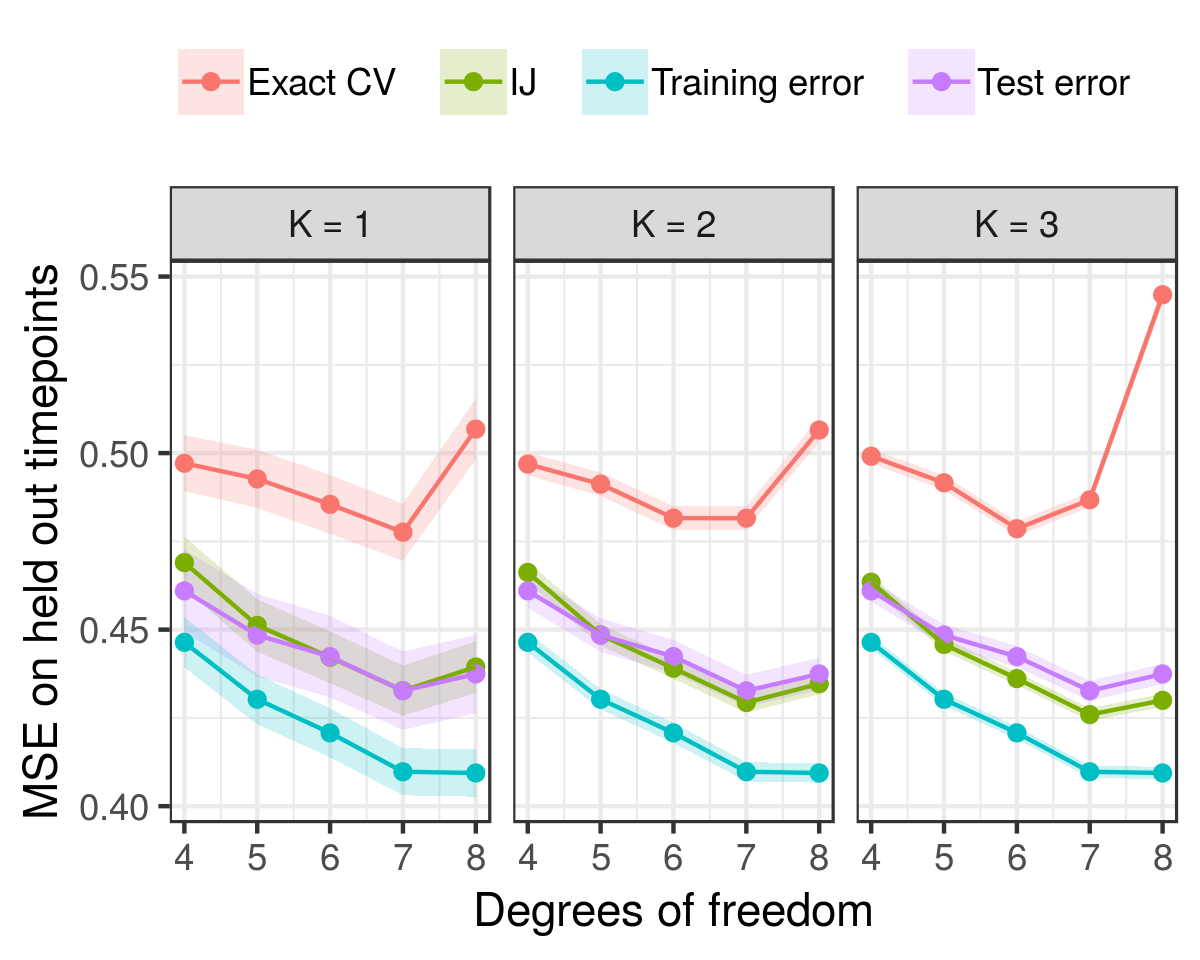
\includegraphics[width=0.98\linewidth,height=0.784\linewidth]{figure/mse_graph-1} 

}

\caption[Genomics data]{Genomics data: accuracy results.}\label{fig:mse_graph}
\end{figure}


\end{knitrout}
%
\fig{mse_graph} shows that the IJ is a reasonably good approximation to the test
set error.\footnote{In fact, in this case, the IJ is a better predictor of test
set error than exact CV.  However, the authors have no reason at present to
believe that the IJ is a better predictor of test error than exact CV in
general.} In particular, both the IJ and exact CV capture the increase in test
error for $df=8$, which is not present in the training error. Thus we see that,
like exact CV, the IJ is able to prevent overfitting. Though the IJ
underestimates exact CV, we note that it differs from exact CV by no more than
exact CV itself differs from the true quantity of iterest, the test error.
%

\begin{knitrout}
\definecolor{shadecolor}{rgb}{0.969, 0.969, 0.969}\color{fgcolor}\begin{figure}[!h]

{\centering 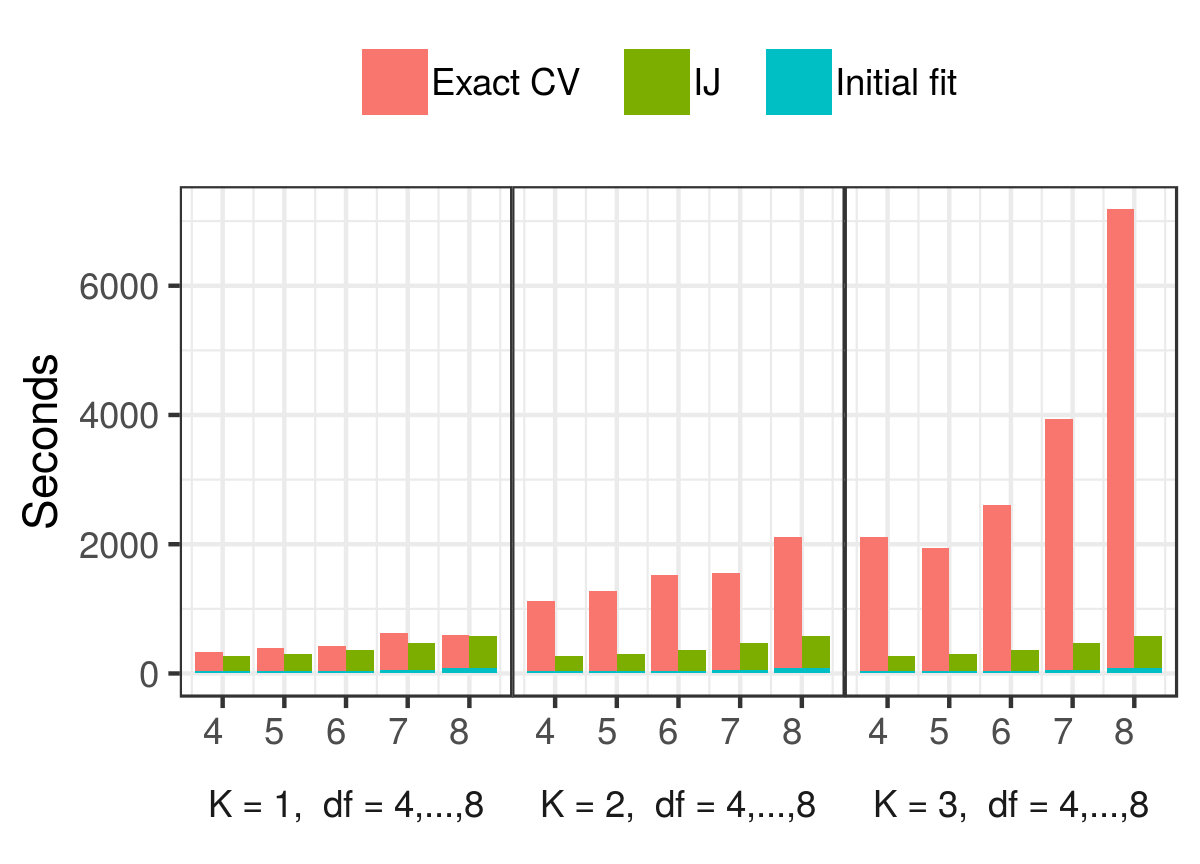
\includegraphics[width=0.98\linewidth,height=0.706\linewidth]{figure/timing_graph-1} 

}

\caption[Genomics data]{Genomics data: timing results.}\label{fig:timing_graph}
\end{figure}


\end{knitrout}
%
The timing results for the genomics experiment are shown in \fig{timing_graph}.
For this particular problem with approximately $\fullparamdim$ parameters (the
precise number depends on the degrees of freedom), finding the initial optimum
takes about $\approxopttime$ seconds. The cost of finding the initial optimum is
shared by exact CV and the IJ, and, as shown in
\fig{timing_graph}, is a small proportion of both.

The principle time cost of the IJ is the
computation of $\hone$. Computing and inverting a dense matrix of size
$\fullparamdim$ would be computationally prohibitive.
But, for the regression objective, $\hone$ is extremely sparse and block diagonal, so computing
$\hone$ in this case took only around $\approxhesstime$ seconds.  Inverting $\hone$
took negligible time. Once we have $\hone^{-1}$, obtaining the
subsequent IJ approximations is nearly instantaneous.

The cost of refitting the model for exact CV varies by degrees of freedom
(increasing degrees of freedom increases the number of parameters) and the
number of left-out points (an increasing number of left-out datapoints increases
the number of refits). As can be seen in \fig{timing_graph}, for low degrees of
freedom and few left-out points, the cost of re-optimizing is approximately the
same as the cost of computing $\hone$.  However, as the degrees of freedom and
number of left-out points grow, the cost of exact CV increases to as much as an
order of magnitude more than that of the IJ.
